%%%%%%%%%%%%%%%%%%%%%%%%%%%%%%%%%%%%%%%%%%%%%%%%%%%%%%%%%%%
% --------------------------------------------------------
% Tau
% LaTeX Template
% Version 2.4.4 (28/02/2025)
%
% Author: 
% Guillermo Jimenez (memo.notess1@gmail.com)
% 
% License:
% Creative Commons CC BY 4.0
% --------------------------------------------------------
%%%%%%%%%%%%%%%%%%%%%%%%%%%%%%%%%%%%%%%%%%%%%%%%%%%%%%%%%%%

\documentclass[9pt,a4paper,twocolumn,twoside]{tau-class/tau}
\usepackage[ngerman]{babel}

%% Draft watermark
% \usepackage{draftwatermark}

% custom Citation commands
\DeclareCiteCommand{\citeauthortitle}
  {\usebibmacro{prenote}}
  {\usebibmacro{citeindex}%
   \printnames{labelname}%
   \setunit{\space\textendash\space}
   \printfield{title}}
  {\multicitedelim}
  {\usebibmacro{postnote}}

  \DeclareCiteCommand{\citeauthortitleurl}
  {\usebibmacro{prenote}}
  {\usebibmacro{citeindex}%
   \printnames{labelname}%
   \setunit{\space\textendash\space}
   \printfield{title}%
   \setunit{\addsemicolon\space}
   \printfield{url}}
  {\multicitedelim}
  {\usebibmacro{postnote}}

\DeclareCiteCommand{\parenciteauthortitle}
  {\usebibmacro{prenote}}
  {\bibopenparen\usebibmacro{citeindex}%
   \printnames{labelname}%
   \setunit{\space\textendash\space}% <- Hier wird das Trennzeichen ":" hinzugefügt
   \printfield{title}\bibcloseparen}
  {\multicitedelim}
  {\usebibmacro{postnote}}

\makeatletter
\renewcommand\footnotesize{\tiny}
\makeatother

\newcommand{\figcite}[1]{\\[0mm]{\tiny Quelle: \cite{#1}}}
\newcommand{\figciteweb}[1]{\\[0mm]{\tiny aus: \citeauthortitle{#1}}}
\newcommand{\figciteweburl}[1]{\\[0mm]{\tiny aus: \citeauthortitleurl{#1}}}

\usepackage{pdfpages}

%----------------------------------------------------------
% TITEL
%----------------------------------------------------------

\journalname{M.Sc. Physik: Spektroskopie}
\title{Second- und Third-Harmonic Generation (SHG/THG) – Grundlagen, Phasenanpassung und Anwendungen}

%----------------------------------------------------------
% AUTOREN, AFFILIATION UND PROFESSOR
%----------------------------------------------------------

\author[a,1]{Florian Marius Adamczyk}

%----------------------------------------------------------

\affil[a]{Justus-Liebig-Universität Gießen, Institut für Physik, Deutschland}

\professor{PD Dr. Arash Rahimi-Iman, Dipl.-Ing.}

%----------------------------------------------------------
% FUSSZEILE
%----------------------------------------------------------

\institution{Justus-Liebig-Universität Gießen}
\footinfo{SHG \& THG Bericht}
\theday{\today}
\leadauthor{Adamczyk, F.}
\course{M.Sc. Physik: Spektroskopie}

%----------------------------------------------------------
% ABSTRACT UND SCHLAGWÖRTER
%----------------------------------------------------------

\begin{abstract}    
In diesem Bericht werden die Grundlagen der Second- und Third-Harmonic Generation (SHG/THG) in der nichtlinearen Optik vorgestellt. Es wird erklärt, wie nichtlineare Polarisation zur Frequenzverdopplung und -verdreifachung führt, welche Rolle die Materialsymmetrie spielt und wie Phasenanpassung (Phase Matching) die Effizienz beeinflusst. Typische experimentelle Aufbauten, Anwendungen (z.B. Mikroskopie) und zentrale Beispiele werden anhand von Abbildungen erläutert.
\end{abstract}

%----------------------------------------------------------

\keywords{SHG, THG, Nichtlineare Optik, Phasenanpassung, Frequenzverdopplung}

%----------------------------------------------------------

\begin{document}
		
    \maketitle 
    \thispagestyle{firststyle} 
    \tauabstract 
    % \tableofcontents
    % \linenumbers 
    
%----------------------------------------------------------

\section{Einleitung und Motivation}
Nichtlineare optische Prozesse ermöglichen es, neue Frequenzen aus intensiven Laserfeldern zu erzeugen. Besonders die Second-Harmonic Generation (SHG) und Third-Harmonic Generation (THG) sind zentrale Effekte, die in der modernen Lasertechnologie, Mikroskopie und Materialanalyse Anwendung finden.

\begin{figure}[!ht]
\centering
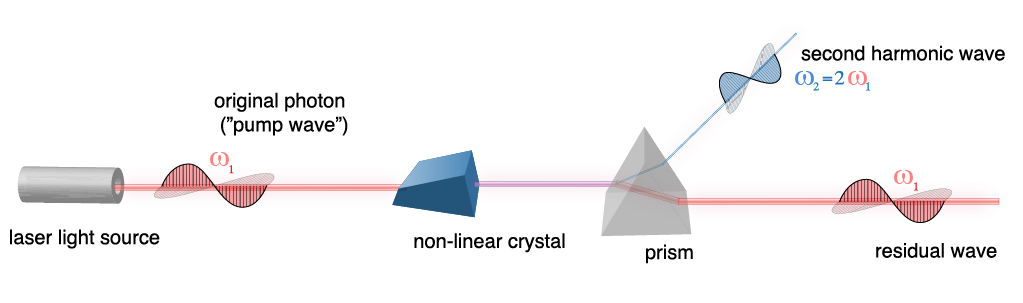
\includegraphics[width=0.6\columnwidth]{figures/experimental.png}
\caption{Schematischer Aufbau für SHG/THG-Experimente.\figcite{JkwchuiImage}}
\end{figure}

%----------------------------------------------------------

\section{Grundlagen der nichtlinearen Optik}
Die Polarisation $P$ eines Mediums als Antwort auf ein elektrisches Feld $E$ lässt sich als Potenzreihe schreiben:
\begin{equation}
P = \varepsilon_0\left[\chi^{(1)}E + \chi^{(2)}E^2 + \chi^{(3)}E^3 + \dots\right]
\end{equation}
Die Terme $\chi^{(2)}$ und $\chi^{(3)}$ beschreiben die nichtlinearen Effekte. $\chi^{(2)}$ ist nur in nicht-zentrosymmetrischen Materialien ungleich null (z.B. viele Kristalle), $\chi^{(3)}$ existiert in allen Medien.

\begin{figure}[!ht]
\centering
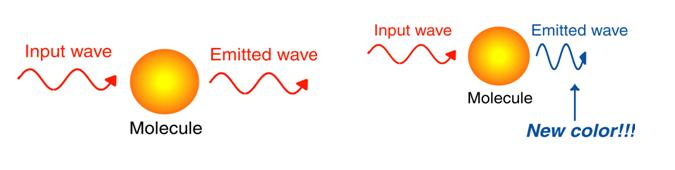
\includegraphics[width=0.6\columnwidth]{../praes/Images/Fig.1 optics.jpeg}
\caption{Links: Lineare, rechts: nichtlineare Antwort eines Mediums auf Licht.\figcite{Science20NonlinearOptics2014}}
\end{figure}

%----------------------------------------------------------

\section{Zweitharmonische Generation (SHG)}
Bei der SHG verschmelzen zwei Photonen der Frequenz $\omega$ zu einem Photon mit $2\omega$. Voraussetzung: $\chi^{(2)} \neq 0$ (keine Inversionssymmetrie).
\begin{equation}
P^{(2)}(2\omega) = \varepsilon_0 \chi^{(2)} E(\omega)^2
\end{equation}

Typische Kristalle: BBO, KTP, KDP, LBO. Effiziente SHG erfordert starke, gepulste Laser und exakte Ausrichtung.

\begin{figure}[!ht]
\centering
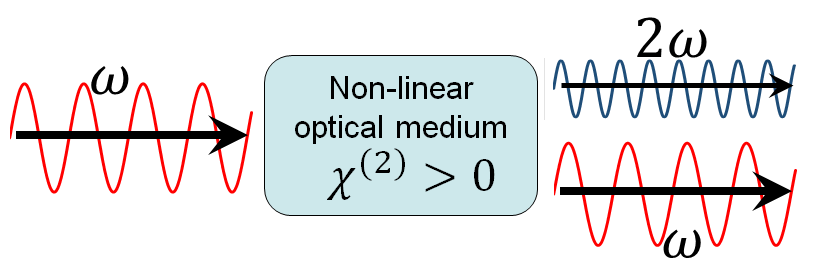
\includegraphics[width=0.6\columnwidth]{../praes/Images/Schematic_of_the_SHG_conversion_of_an_excited_wave_in_a_non-linear_medium.png}
\caption{Schematische Darstellung: Einfallende Welle erzeugt zweite Harmonische im nichtlinearen Medium.\figciteweburl{BPAegirsson2017}}
\end{figure}

Historisch wurde SHG erstmals 1961 mit einem Rubinlaser beobachtet (Franken et al.).

%----------------------------------------------------------

\section{Drittharmonische Generation (THG)}
Bei der THG verschmelzen drei Photonen $\omega$ zu einem Photon $3\omega$. $\chi^{(3)}$ ist in allen Materialien vorhanden, daher ist THG auch in Flüssigkeiten und Gasen möglich.
\begin{equation}
P^{(3)}(3\omega) = \varepsilon_0 \chi^{(3)} E(\omega)^3
\end{equation}

\begin{figure}[!ht]
\centering
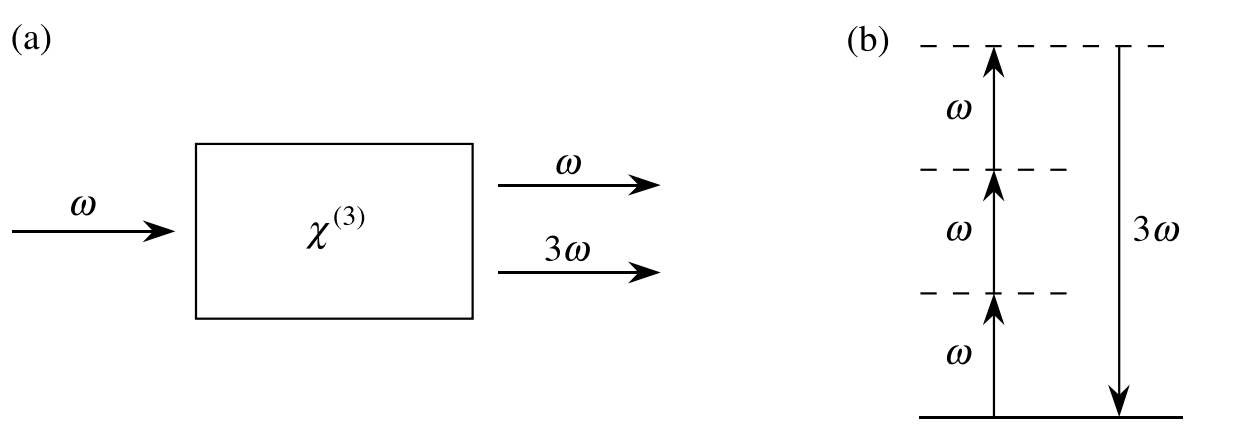
\includegraphics[width=0.95\columnwidth]{../praes/Images/thg.png}
\caption{Drei Photonen $\omega$ erzeugen ein Photon $3\omega$.\figciteweb{Boyd2020}}
\end{figure}

THG ist meist schwächer als SHG, aber besonders effektiv an Grenzflächen oder bei Brechungsindexgradienten (z.B. THG-Mikroskopie).

%----------------------------------------------------------

\section{Nichtlineare Suszeptibilität und Symmetrie}
Ob ein Material SHG zeigt, hängt von der Symmetrie ab. In zentrosymmetrischen Medien verschwindet $\chi^{(2)}$, nur $\chi^{(3)}$ bleibt.

\begin{figure}[!ht]
\centering
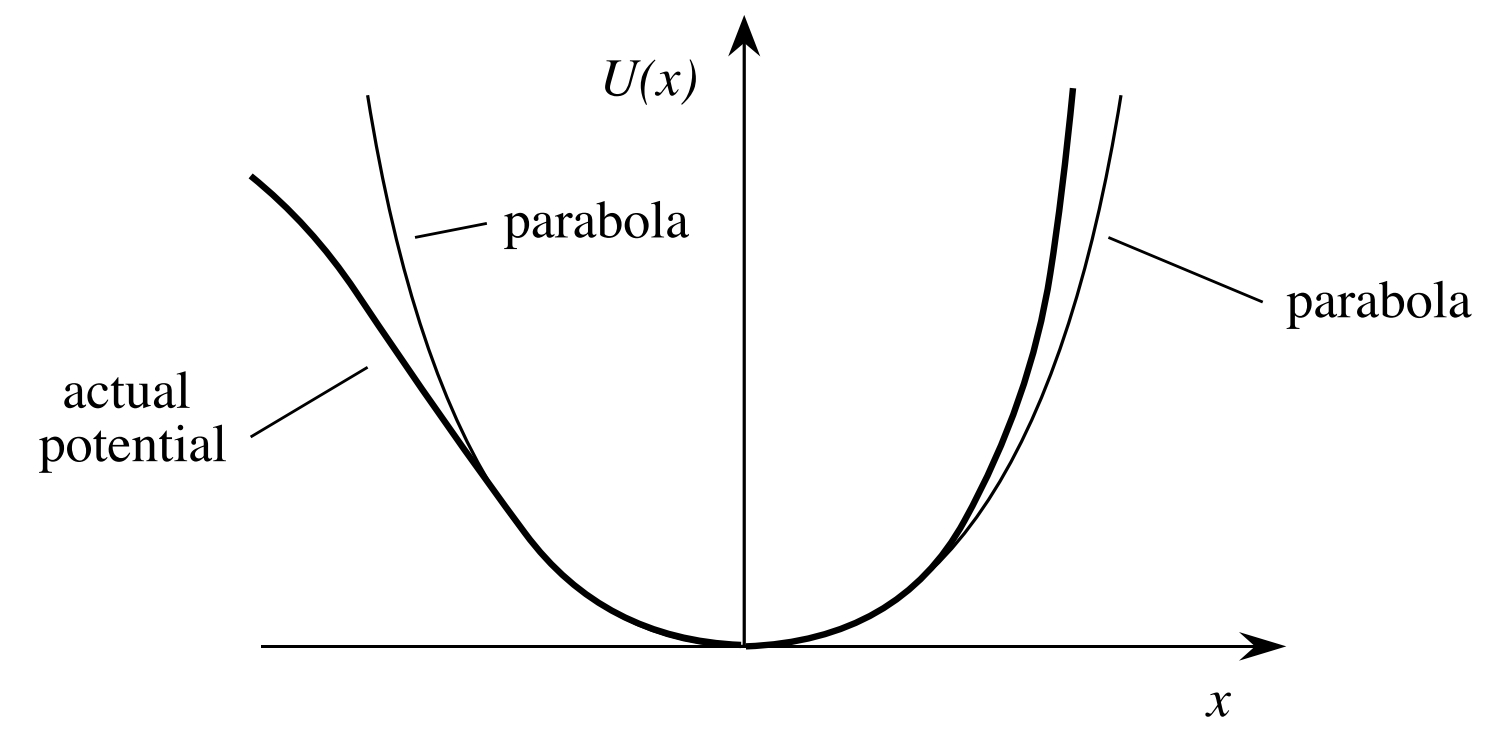
\includegraphics[width=0.45\columnwidth]{../praes/Images/pot_noncentrosym.png}
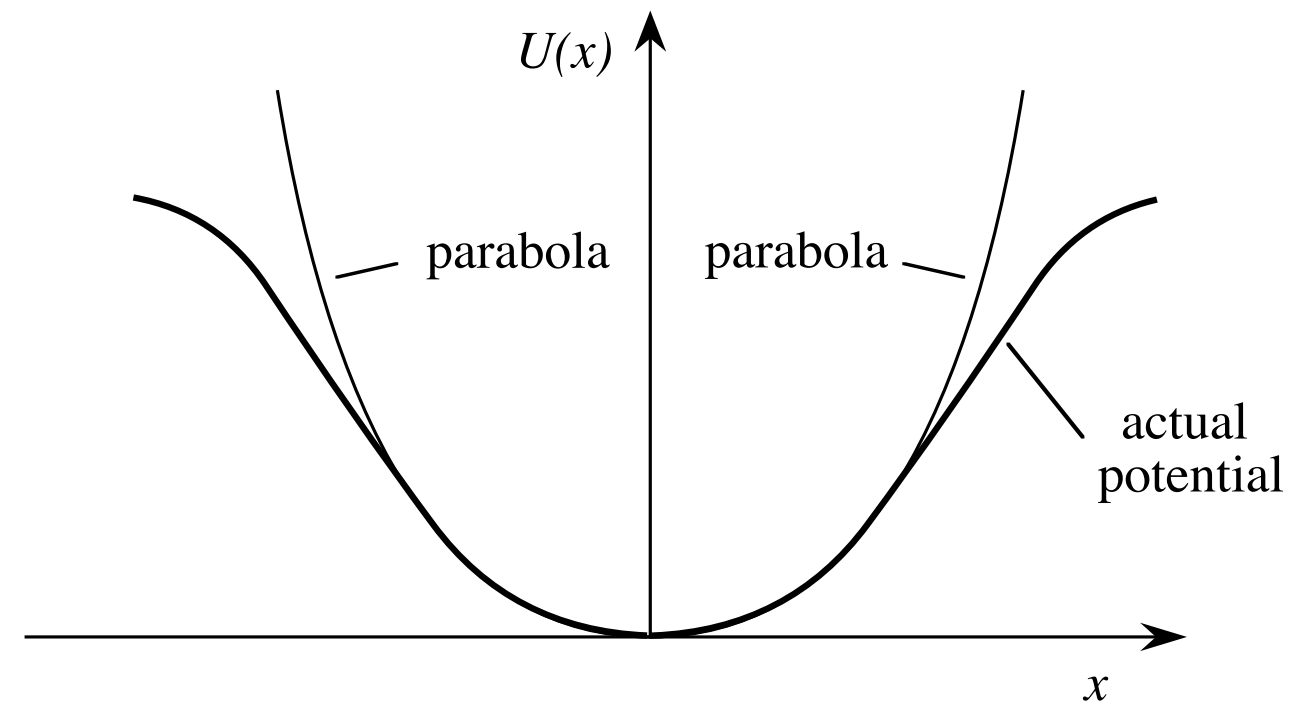
\includegraphics[width=0.45\columnwidth]{../praes/Images/pot_centrosym.png}
\caption{Links: Potential ohne Inversionssymmetrie ($\chi^{(2)} \neq 0$), rechts: mit Inversionssymmetrie ($\chi^{(2)} = 0$).\figcite{Boyd2020}}
\end{figure}

%----------------------------------------------------------

\section{Phasenanpassung (Phase Matching)}
Für effiziente Frequenzkonversion müssen Grund- und Harmonische phasenkohärent bleiben. Dies wird durch Doppelbrechung (Birefringenz) oder periodische Polung erreicht.

\begin{figure}[!ht]
\centering
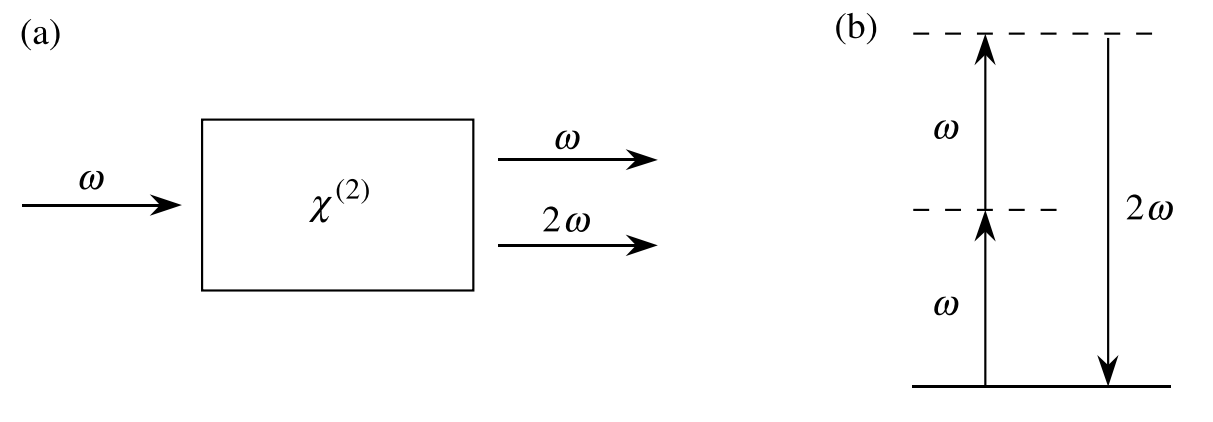
\includegraphics[width=0.98\columnwidth]{../praes/Images/shg.png}
\caption{SHG: $\omega \rightarrow 2\omega$. Die Grafik illustriert die Energieumwandlung.\figcite{Boyd2020}}
\end{figure}



%----------------------------------------------------------

\section{Experimenteller Aufbau und Anwendungen}
Ein typischer Aufbau besteht aus Laser, nichtlinearem Kristall, Strahlführung, Filtern und Detektor.

\begin{figure}[!ht]
\centering
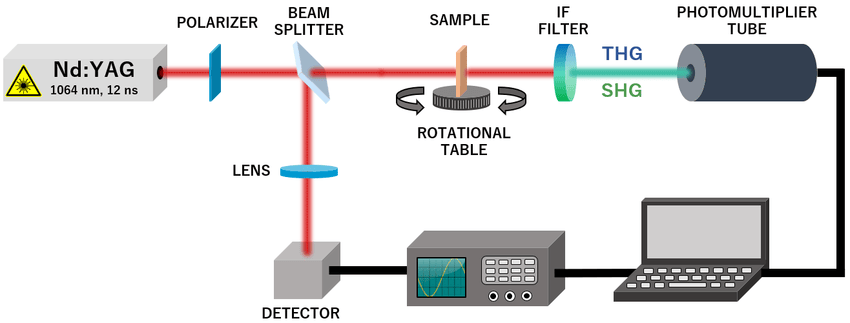
\includegraphics[width=0.95\columnwidth]{../praes/Images/Experimental-setup-measuring-SHG-and-THG-intensity-relative-to-laser-energy.png}
\caption{Experimenteller Aufbau zur Messung der SHG- und THG-Intensität in Abhängigkeit von der Laserenergie.\figciteweburl{ResearchGate2025}}
\end{figure}

\subsection{SHG-Mikroskopie}
SHG-Mikroskopie nutzt die nichtlineare Antwort von Strukturen wie Kollagen für kontrastreiche, markerfreie Bildgebung in der Biologie.

\subsection{Weitere Anwendungen}
\begin{itemize}
    \item Frequenzverdopplung in Lasern (z.B. grüne Laserpointer)
    \item Materialcharakterisierung
    \item Oberflächenanalytik (z.B. SHG an Grenzflächen)
\end{itemize}

%----------------------------------------------------------

\section{Zusammenfassung und Ausblick}
SHG und THG sind fundamentale Prozesse der nichtlinearen Optik. Die Effizienz hängt von Material, Symmetrie und Phasenanpassung ab. Anwendungen reichen von der Lasertechnik bis zur Biophysik.

%----------------------------------------------------------

\section{Komponenten und Messung}
Die wichtigsten Komponenten eines SHG/THG-Experiments sind:
\begin{itemize}
    \item \textbf{Laser:} Pulsdauer, Wellenlänge, Leistung (z.B. Nd:YAG 1064 nm, Ti:Sa 800 nm)
    \item \textbf{Kristall:} Material (BBO, KTP, LBO), Dicke, Temperatur, Ausrichtung
    \item \textbf{Strahlführung:} Polarisation, Fokussierung auf den Kristall
    \item \textbf{Filter:} Blockieren das Grundsignal, lassen nur die Harmonische durch
    \item \textbf{Detektor:} Photodiode oder Spektrometer
\end{itemize}
Die Intensität der erzeugten Harmonischen wird typischerweise gegen die Eingangsleistung oder den Kristallwinkel gemessen. Für SHG ist die Abhängigkeit quadratisch ($I_{SHG} \propto P^2$), für THG kubisch.


%----------------------------------------------------------

\section{Weitere Spezialfälle und Prozesse}
\subsection{Sequential THG und HHG}
Bei Sequential THG erfolgt die Frequenzverdreifachung in mehreren Stufen ($\omega \rightarrow 2\omega \rightarrow 3\omega$). High Harmonic Generation (HHG) ist ein nichtlinearer, nichtperturbativer Prozess, der sehr hohe Ordnungen ermöglicht.

\subsection{Sum-Frequenz- und Differenz-Frequenz-Generation (SFG/DFG)}
SFG: Zwei Photonen unterschiedlicher Frequenz ($\omega_1$, $\omega_2$) erzeugen ein Photon mit $\omega_3 = \omega_1 + \omega_2$. Beide Prozesse benötigen starke Felder und Phasenanpassung.

\subsection{SHG vs. Zweiphotonenabsorption (TPA)}
SHG ist ein kohärenter Prozess, bei dem zwei Photonen zu einem neuen Photon verschmelzen. TPA ist ein inkohärenter Prozess, bei dem zwei Photonen gleichzeitig absorbiert werden, um ein Elektron anzuregen.

%----------------------------------------------------------

\section{Beispiele und Anwendungen}
\begin{itemize}
    \item \textbf{Grüne Laserpointer:} SHG aus IR-Laser (1064 nm) erzeugt sichtbares Licht (532 nm)
    \item \textbf{Materialcharakterisierung:} Bestimmung von $\chi^{(2)}$ und $\chi^{(3)}$
    \item \textbf{Oberflächenanalytik:} SHG ist sensitiv für nicht-zentrosymmetrische Bereiche (z.B. Grenzflächen, Adsorbate)
    \item \textbf{Biologische Bildgebung:} SHG- und THG-Mikroskopie für label-freie, kontrastreiche Aufnahmen (z.B. Kollagen, Zellmembranen)
\end{itemize}

\begin{figure}[!ht]
\centering
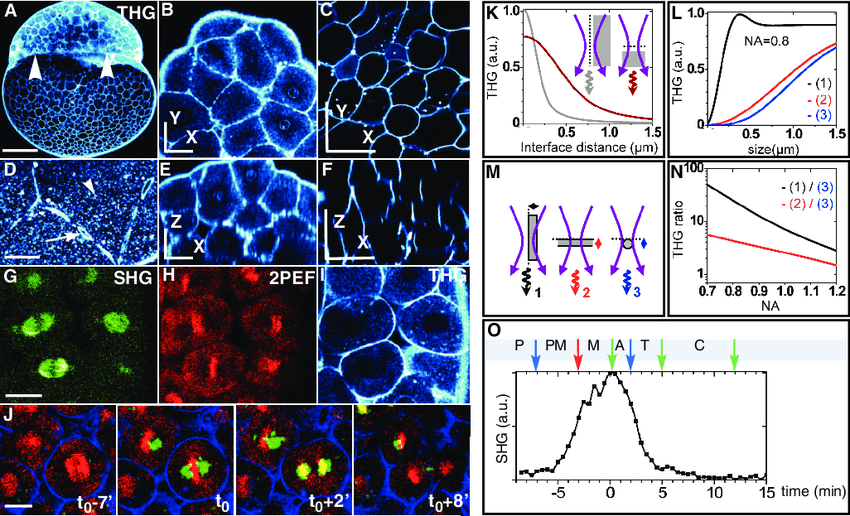
\includegraphics[width=0.6\columnwidth]{../praes/Images/THG-and-SHG-signals-in-the-zebrafish-embryo-during-cleavage-stages-A-Sagittal-THG.png}
\caption{SHG/THG-Mikroskopie am Zebrafisch-Embryo.\figciteweb{ResearchGateZebrafish2009}}
\end{figure}

%----------------------------------------------------------

\printbibliography % Literaturverzeichnis

%----------------------------------------------------------

% \section*{Anhang}
% Im Anhang sind beispielhafte LLM-Konversationen dokumentiert, die zur Erstellung dieses Berichts genutzt wurden.

% 
\includepdf[pages=-]{LLM_documentation/001.pdf}
% 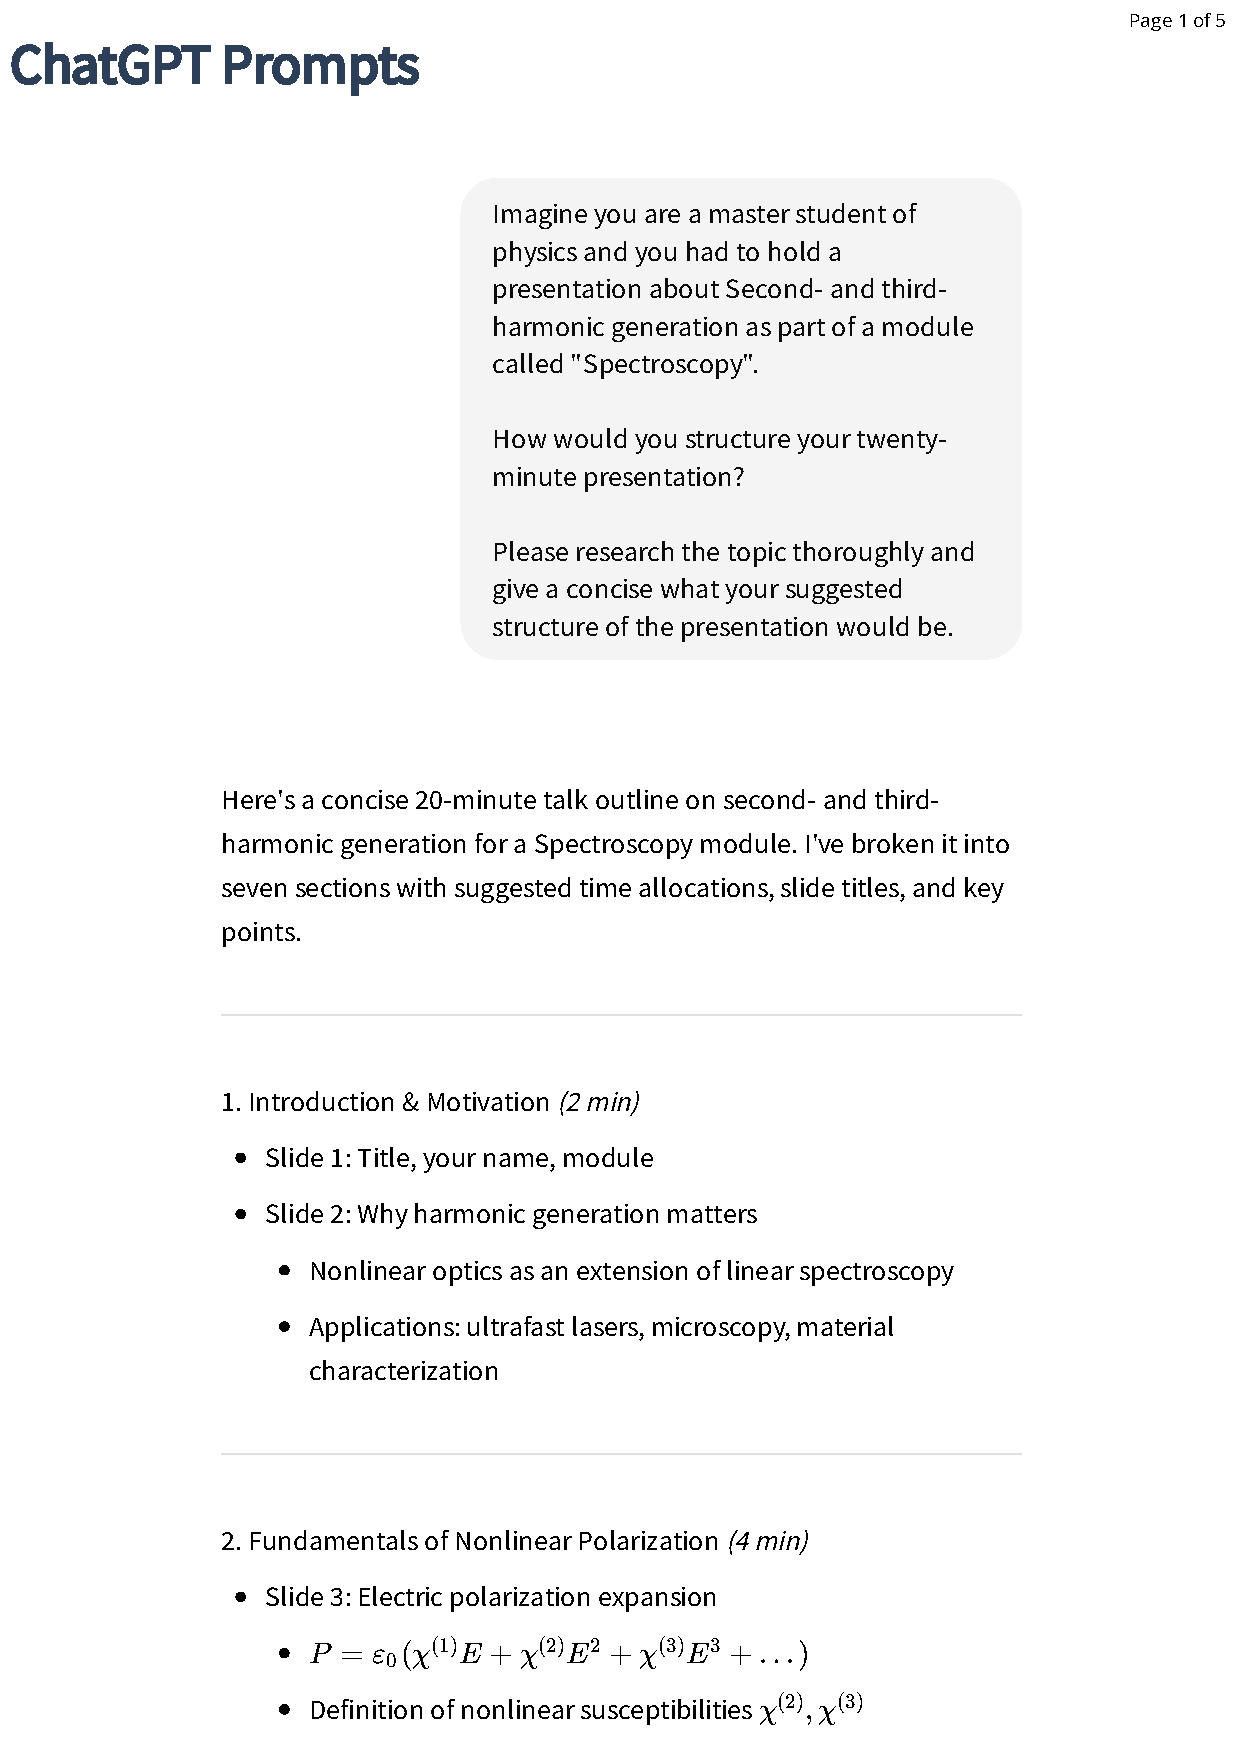
\includepdf[pages=-]{LLM_documentation/+01.pdf}
% 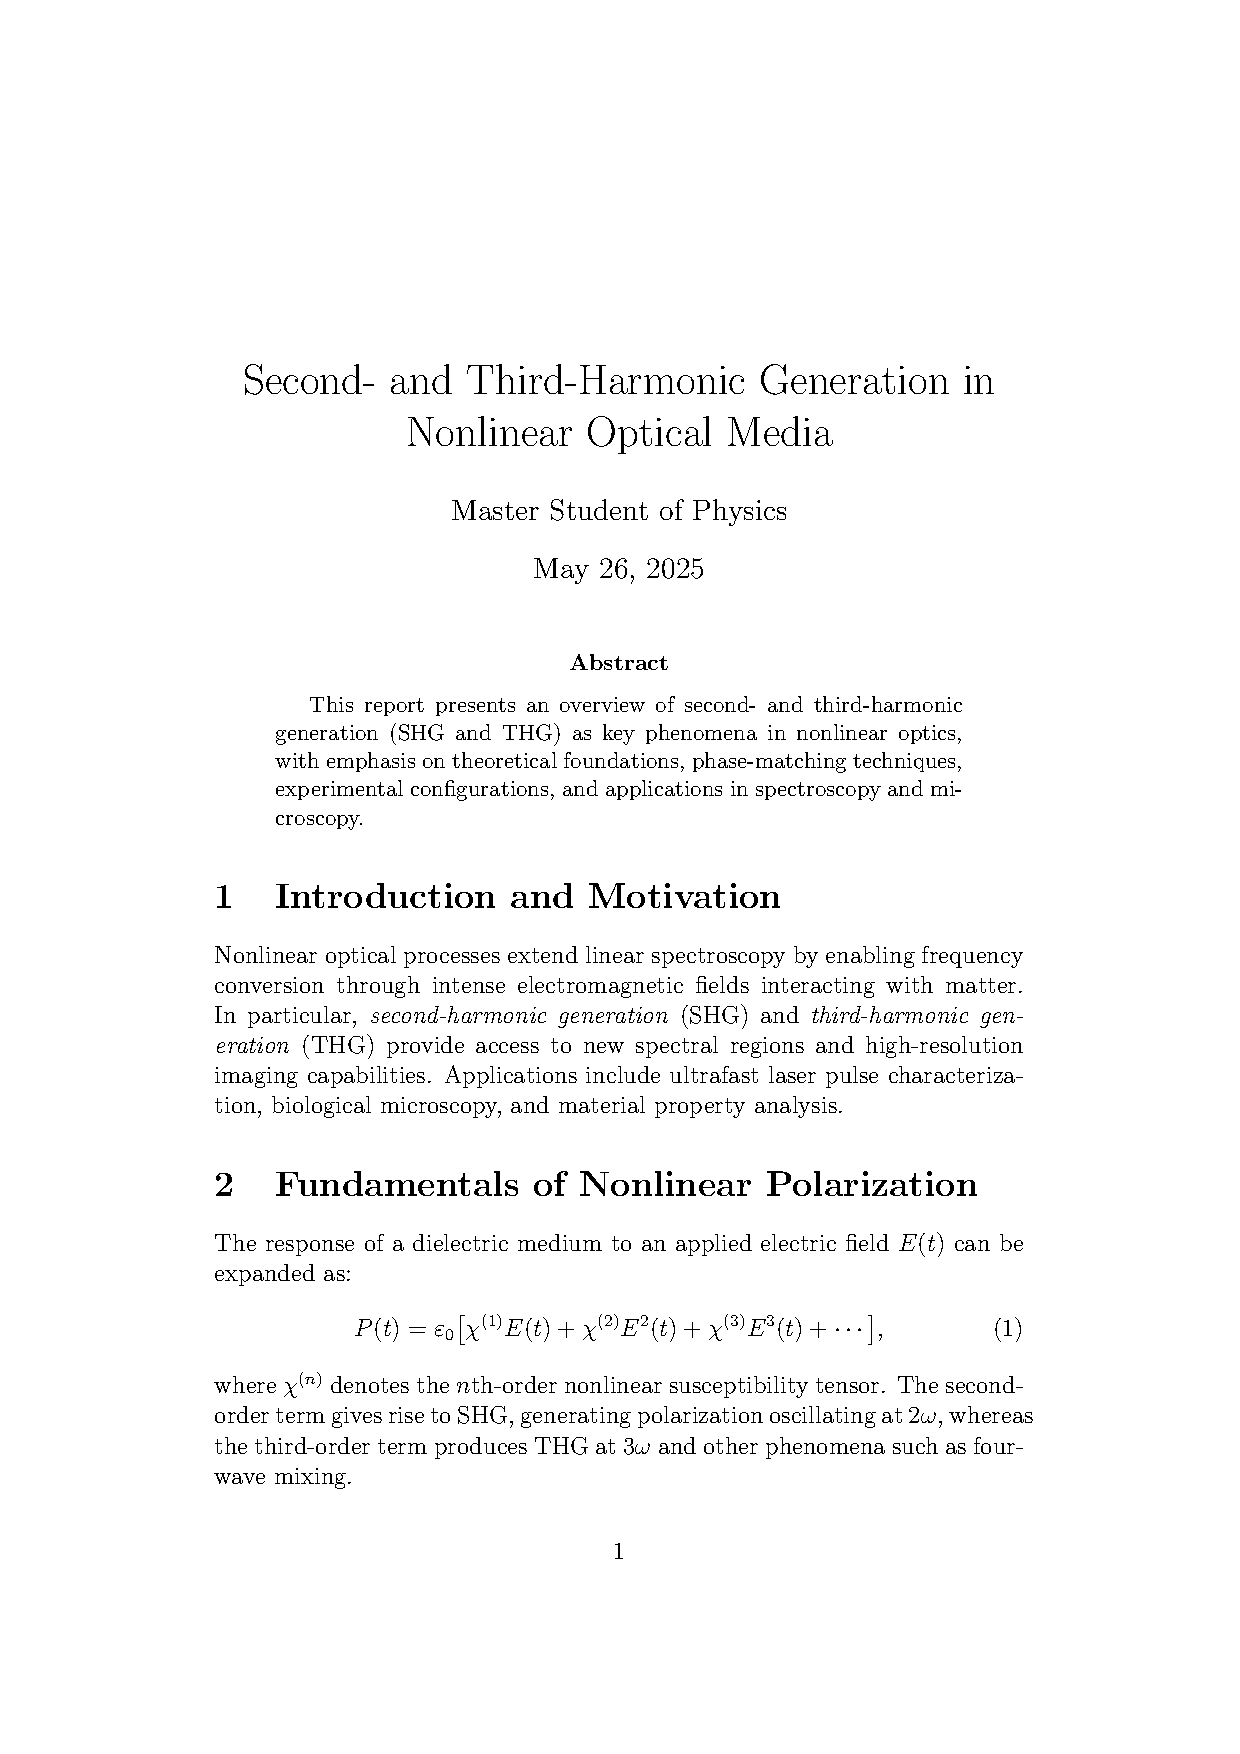
\includepdf[pages=-]{LLM_documentation/FirstTest/firstTest.pdf}

\end{document}